\chapter{Methodology}\
\section{AMS at Aarhus University}
When measuring isotopic ratios of stable nuclei, such as isotopes, conventional mass spectrometry is sufficiently proficient, providing adequate sensitivity Refs. \cite{steinhof2016}, \cite{tuniz1998ams}.

However, to measure cosmogenic nuclei such as \ce{^{10}Be}, with isotopic ratios between $10^{-10}$ and $10^{-14}$, the limitations of conventional mass spectrometers are surpassed. Utilizing AMS allows access to higher energies, which in turn helps resolve ambiguities in identifying nuclei, atoms, and molecular ions of the same mass.\ As described in the section Principles of AMS, the setup at Aarhus University follows a similar configuration. The AMS system for AARAMS is composed of several components, which will be described in this section along with their effects on the ion beam. The schematic layout of AARAMS, depicted in  \cref{fig:AuAMS}, shows that it can be divided into five "main" sections: Ion source, Low Energy section (LE), \ce{1MV} accelerator, High Energy section (HE), and the Rare Isotope section (RI), followed by the detector.

Additionally, the optical beam-handling components include Einzellenses, Y- and X-steerers, X-slits, apertures, Q-snout lenses, and Q-pole lenses, as well as retractable Faraday cups for measuring and analyzing the beam current.

\begin{figure}
    \centering
    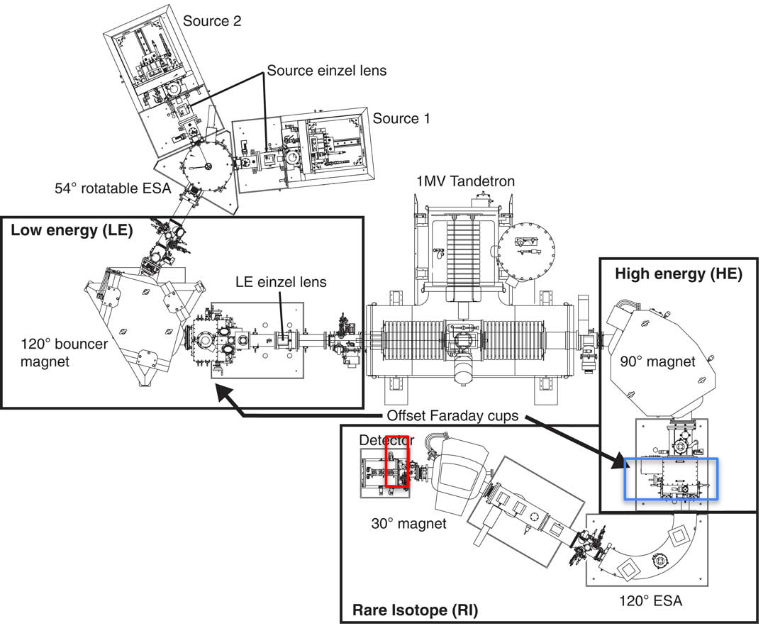
\includegraphics[width=\textwidth]{B/AarhusAMSTecDraw.PNG}
    \caption{A 5-sub division of the \ce{1 MV} Tandetron Accelerator layout at Aarhus University Ref.\cite{olsen2017}. The blue rectangle is where foils can be slit down to intersect the beam. The red rectangle is where we will add \ce{SiN} foils, as suggested by Ref. \cite{steier2019}. The latter rectangles represent two different setups.} 
    \label{fig:AuAMS}
\end{figure}

\subsection{Ion Source}

The first section in the AARAMS is essentially where the beam of \ce{^{10}Be}, and other ions, is created. Inserting \ce{^{10}Be} directly for analysis is not possible, due to its extremely low abundance, as well as doing so will contaminate the beam. The samples used are cathodes made out of copper - due to its electron affinity of \ce{118.4 \frac{kJ}{mol}} Ref.\cite{web_elements_copper}- containing on average \ce{0.7142} \ce{\pm 0.0761 mg}
\ce{^{10}Be^{16}O}, beryllium oxide, which is sometimes referred to as  "beryllia" see \cref{Betable}. 
The average weight of BeO was calculated using:
\begin{equation}
\text{Average BeO mass} = \frac{\sum \text{BeO weights}}{N} \quad (N = 12)
\end{equation}
where \( N \) is the total number of samples.
The uncertainty was calculated using the standard deviation \( s \) of the weights:
\begin{equation}
s = \sqrt{\frac{\sum (x_i - \text{average})^2}{N-1}} \quad \text{and} \quad \text{Uncertainty} = \frac{s}{\sqrt{N}}
\end{equation}
Similar calculations are done for Niobium yielding an average mass of \ce{m_{Nb}=3.585}\ce{\pm 0.253mg}.

\begin{table}[ht]
    \centering
    \caption{\ce{^{10}Be} Batch Information}
    \resizebox{\linewidth}{!}{ % Resize the table to fit the linewidth
    \begin{tabular}{@{}llcccccccc@{}} % Removed the last 'c' for the comments column
        \toprule
        Sample Name & Sample Type & Batch & Sample origin & Description of Carrier & Preparation Lab & Lab prep & Registration date & BeO mass (mg) & Nb added (mg) & mixing-ratios \\ \midrule
        AU2406 & pblk & AU2406 & MFK/Katya & PHE1603 & AARGEO & BE & 9/17/2024 & 0.62 & 2.81 & 4.5 \\
        RUB20 & sam & AU2406 & MFK/Katya & PHE1603 & AARGEO & BE & 9/17/2024 & 1.35 & 5.53 & 4.1 \\
        RUB21 & sam & AU2406 & MFK/Katya & PHE1603 & AARGEO & BE & 9/17/2024 & 0.27 & 2.29 & 8.5 \\
        RUB22 & sam & AU2406 & MFK/Katya & PHE1603 & AARGEO & BE & 9/17/2024 & 1.07 & 4.51 & 4.2 \\
        RUB23 & sam & AU2406 & MFK/Katya & PHE1603 & AARGEO & BE & 9/17/2024 & 0.76 & 4.00 & 5.3 \\
        RUB24 & sam & AU2406 & MFK/Katya & PHE1603 & AARGEO & BE & 9/17/2024 & 0.79 & 3.28 & 4.2 \\
        RUB26 & sam & AU2406 & MFK/Katya & PHE1603 & AARGEO & BE & 9/17/2024 & 0.72 & 3.77 & 5.2 \\
        RUB27 & sam & AU2406 & MFK/Katya & PHE1603 & AARGEO & BE & 9/17/2024 & 0.79 & 3.43 & 4.3 \\
        RUB28 & sam & AU2406 & MFK/Katya & PHE1603 & AARGEO & BE & 9/17/2024 & 0.73 & 2.95 & 4.0 \\
        RUB29 & sam & AU2406 & MFK/Katya & PHE1603 & AARGEO & BE & 9/17/2024 & 0.93 & 3.72 & 4.0 \\
        Cosmo1 & sam & AU2406 & MFK/Katya & PHE1603 & AARGEO & BE & 9/17/2024 & 0.60 & 2.84 & 4.7 \\
        C0-34 & sam & AU2406 &  & PHE1603 & AARGEO & BE & 9/17/2024 & 0.57 & 2.80 & 4.9 \\ \bottomrule
    \end{tabular}}
    \label{Betable}
\end{table}

The type of ion source used at the AARAMS is a cesium sputter source, as described above. The AARAMS has two independently operable negative ion sources, HVEE SO-110C-1 (source 1) and SO-110C-2 (source 2), each capable of holding up to 50 samples. This allows for a quick switch between samples, which is admirable.

At AARAMS, cesium vapor is first heated to approximately $\ce{115^{\circ}C}$ in a boiler and directed into an ionization cavity maintained at around $\ce{1000^{\circ}C}$, enabling efficient ionization because of cesium’s low first ionization energy out of all the elements Ref.\cite{mcmurry2018}. The cavity’s ionizer, heated to $\ce{1100^{\circ}C}$ by passing a current of approximately \ce{18 A} through an embedded coil, releases electrons, which interact with cesium atoms to create Cs+ ions. The generated cations are focused and accelerated towards the sample containing \ce{BeO} to sputter its surface, creating a beam of anions. The adjustable length of the sample holder allows for precise positioning of the sample relative to the focal point, optimizing sputtering efficiency. At AARAMS, the target voltage and extraction voltage sum are set to \ce{35 kV}, with a constraint of \ce{\pm3 kV} due to limitations in the bouncer injector magnet.

The beam of anions, consisting of molecules such as \ce{^{10}Be^{16}O^{-}}, is subjected to uniform acceleration, resulting in equal kinetic energy for each ion. This ensures that all ions in the beam, regardless of their mass or charge, attain the same kinetic energy under these conditions. They are accelerated towards a rotatable ESA.

The ESA is a $\ce{54^{\circ}}$ electrostatic analyzer with a radius of \ce{469 mm}, a gap of \ce{53 mm}, and an energy-to-charge ratio of \ce{44 kV} \cite{HVEE2013}. The ESA can be seen in \cref{fig:ESA54}, where two curved, parallel conducting plates create a radial electric field of strength $\mathcal{E}$ between them. 

\begin{figure}[ht]
    \centering
    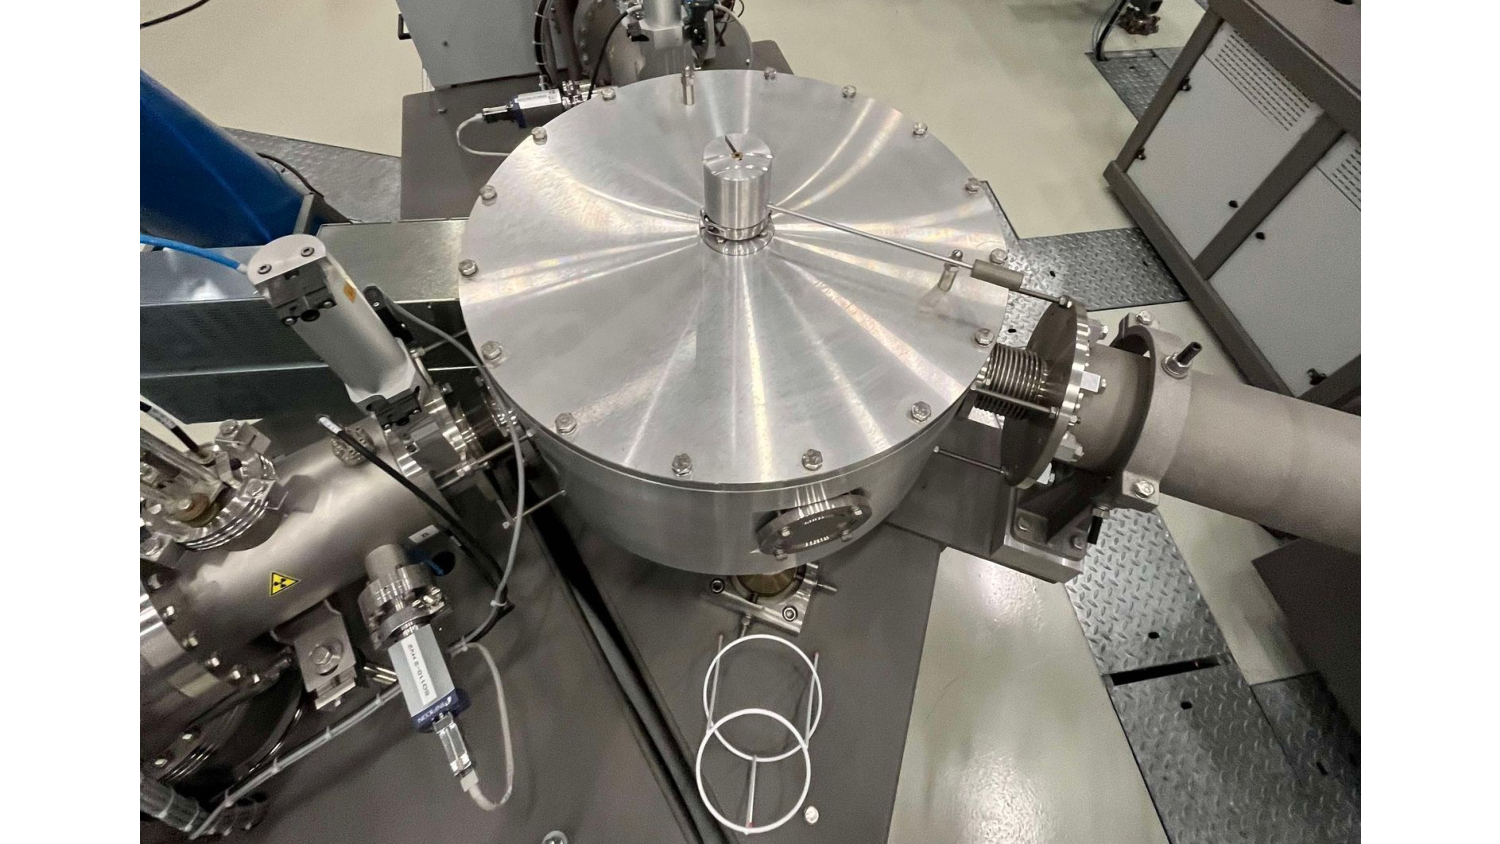
\includegraphics[width=1\linewidth]{B/ESA1.pdf}
    \caption{Rotatable $54^{\circ}$ Electrostatic analyzer.}
    \label{fig:ESA54}
\end{figure}



The ESA guides ions along a circular path, allowing only those with specific energy levels to pass through by setting the arc radius, $r$, according to the ions’ energy-to-charge ratio, as described in \cref{electricrigitidy}. The electrodes are held at equal voltages but with opposite polarities \cite{HVEE2013}. Given the electrostatic rigidity of an ion, $e$, the required voltage on one of the ESA electrodes can be calculated as:

\begin{equation}
    \mathcal{V}_{ESA} = \frac{E_{i} \, x_{\text{gap}}}{q \, r}
\end{equation}

where the ion's energy, $E_i$, the gap between the electrodes, $x_{\text{gap}}$, the ion's charge, $q$, and the radius of curvature, $r$, are used in the calculation.

%\subsection{LE Section}
%When their electrostatic rigidity in the ESA has sorted the beam of ions, they will proceed towards the $\ce{120^{\circ}}$ BI magnet with a radius of 455 mm, with a gap of approximately 62 mm capable of producing a mass-energy production of \ce{12AMU-MeV}. The charged particles in the ion beam will be analyzed by their magnetic rigidity whose ratio is given by \cref{magnetrigitidy}.The magnets at AARAMS are equipped with Hall probes. These are calibrated Hall effect sensors, that utilize how charged particle-field dynamics work. The Hall effect is when an electric current flows through a conducting material in the presence of a magnetic field, the magnetic field induces the Lorentz force upon the moving electrons. This deflection of electrons results in the accumulation of electrons on one side of the conductor, thereby inducing a potential difference between both sides of the conductor. This potential difference can be measured and is known as the Hall voltage and is correctly correlated to the hall probe Refs.\cite{wiki:hall_effect_sensor}, \cite{electronics:tutorial_hall_effect}.

\subsection{LE section}

In the LE section, ions are sorted and directed based on their energy and charge before entering the accelerator. The crucial elements here include the ESA and the bouncer magnet, which help separate and direct ion beams of different masses through the accelerator.

When the electrostatic rigidity of the ions has been adjusted by the ESA, the ion beam is guided through a $\ce{120^{\circ}}$ bouncer magnet. The bouncer magnet, with a 455 mm radius and a gap of approximately 62 mm. By controlling the magnetic rigidity whose ratio is given by \cref{magnetrigitidy}, the trajectory of the charged particles in the ion beam will be determined.

To ensure that ion beams of different masses follow the same trajectory through the bouncer magnet, we must adjust the bouncer voltage, ensuring the same magnetic rigidity for all ions in the beam. This is crucial because beams of differing masses would otherwise follow different paths in the BI magnet. The relationship between two ion beams, one of a reference mass and the other of a different mass, is governed by the equality in their magnetic rigidity this could be for \ce{^{9}Be} and \ce{^{10}Be}

\begin{equation*}
    \dfrac{p\left(\ce{^{9}Be}\right)}{q\left(\ce{^{9}Be}\right)}=\dfrac{p\left(\ce{^{10}Be}\right)}{q\left(\ce{^{10}Be}\right)}
\end{equation*}

and by substituting the momentum as defined in \cref{Magnetssection} allows us to determine how the bouncer voltage should be adjusted to ensure the same path for both beams

\begin{equation}
    \sqrt{\dfrac{2m_{9}E_{9}}{q\left(\ce{^{9}Be}\right)^{2}}}=    \sqrt{\dfrac{2m_{10}E_{10}}{q\left(\ce{^{10}Be}\right)^{2}}}
\end{equation}

This equation can be used to tune the bouncer voltage settings such that ion beams of different masses,\ce{^{9}Be} and \ce{^{10}Be}, will leave the bouncer magnet following the same trajectory.

\subsubsection{Hall effect and magnetic monitoring}
To ensure precise control of the magnetic field in the bouncer magnet, the system at AARAMS employs Hall probes. These are calibrated sensors that utilize the Hall effect to monitor the strength of the magnetic field within the magnet. The Hall effect occurs when a magnetic field is applied perpendicular to a current flowing through a conductor, causing a Lorentz force to deflect the electrons and accumulate charge on one side of the conductor. This accumulation results in a voltage difference, called the Hall voltage, which is proportional to the magnetic field strength \cite{wiki:hall_effect_sensor, electronics:tutorial_hall_effect}.

The Hall voltage $V_{H}$ is given by
\begin{equation}
    V_H = \frac{I B}{n e d_{c}}
    \label{hallvoltage}
\end{equation}

where $I$ is the current through the conductor, $B$ is the magnetic field strength, $n$ is the charge carrier density, $e$ is the electron charge, $d_{c}$ is the thickness of the conductor.

By continuously measuring the Hall voltage, we can monitor the magnetic field in real-time, ensuring that it remains at the correct strength to direct the ion beam along its intended trajectory. This is particularly important for ensuring that the beam of ions, such as \ce{^{9}Be} and \ce{^{10}Be}, is precisely focused as it exits the bouncer magnet and proceeds to the accelerator.

To match the trajectory of beams with different masses, the bouncer voltage \( V_{\text{BNC}} \) must be tuned accordingly. The reference beam, with mass \( m_{\text{REF}} \), has a reference bouncing voltage \( V_{\text{REF}} \), which is typically set to zero. For a beam of mass \( m_{\text{BNC}} \), the energy equation can be expressed as:

\begin{equation}
    m_{\text{BNC}}  q  (V_{\text{Tar}} + V_{\text{Ex}} + V_{\text{BNC}}) = m_{\text{REF}}  q  (V_{\text{Tar}} + V_{\text{Ex}} + V_{\text{REF}})
\end{equation}

Isolating for \( V_{\text{BNC}} \), we get:

\begin{equation}
    V_{\text{BNC}} = (V_{\text{Tar}} + V_{\text{Ex}} + V_{\text{REF}})  \frac{m_{\text{REF}}}{m_{\text{BNC}}} - (V_{\text{Tar}} + V_{\text{Ex}})
\end{equation}

This equation determines the bouncer voltage necessary to ensure that beams with different masses follow the same trajectory through the bouncer magnet, allowing for precise acceleration and injection into the accelerator \cite{HVEE2013}.


\subsection{\ce{1$\MV$} Accelerator Section}
\Cref{fig:acceleratorphoto.pdf}  provides a view of the 1$\MV$ tandem accelerator at AARAMS, highlighting the entry point for the cation beam, which has been sorted by energy, charge, and mass.

\begin{figure}[ht] \centering 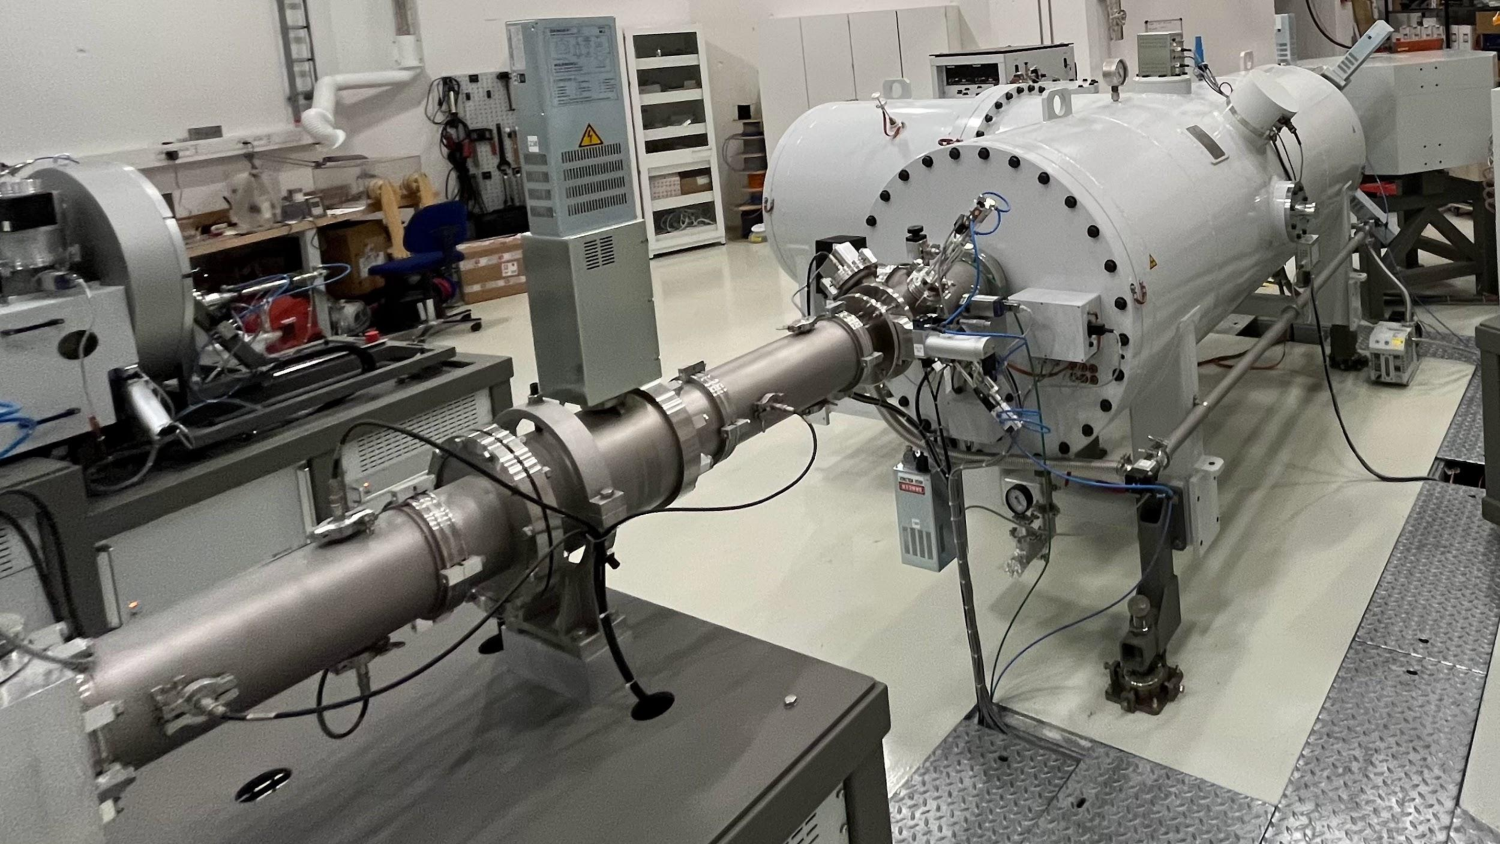
\includegraphics[width=\linewidth]{B/acceleratorphoto.pdf} \caption{The \ce{1$\MV$} tandem accelerator at AARAMS, showing the entry pipe where the ion beam enters the accelerator.} \label{fig:acceleratorphoto.pdf} \end{figure}

To understand the accelerator at AARAMS, it is important to be familiar with its main components: an insulating tank filled with \ce{SF6} gas, low- and high-energy accelerator tubes, a Cockcroft-Walton voltage multiplier, and a charge-exchange chamber equipped with gas, pressure gauges, and various beam-handling elements, including Q-snout and Q-pole lenses. This section plays a critical role in determining the charge state and energy distribution of ions as they move toward the FC and detector. At the core of the AARAMS accelerator lies a gas-exchange tube, commonly referred to as the "stripper," which enables dual acceleration of ions within a single voltage potential.

The stripper dissociates complex molecular ions, such as \ce{BeO-}, reducing their intensity and converting anions into cations. This process allows smaller molecular fragments to be filtered out in subsequent stages, though it typically reduces the overall beam intensity \cite{weisser2005stripper}.

At the center of the accelerator chamber, the terminal acceleration potential is generated by a Cockcroft-Walton (CW) multiplier, which is schematically depicted in \cref{fig
}.

\begin{figure} \centering 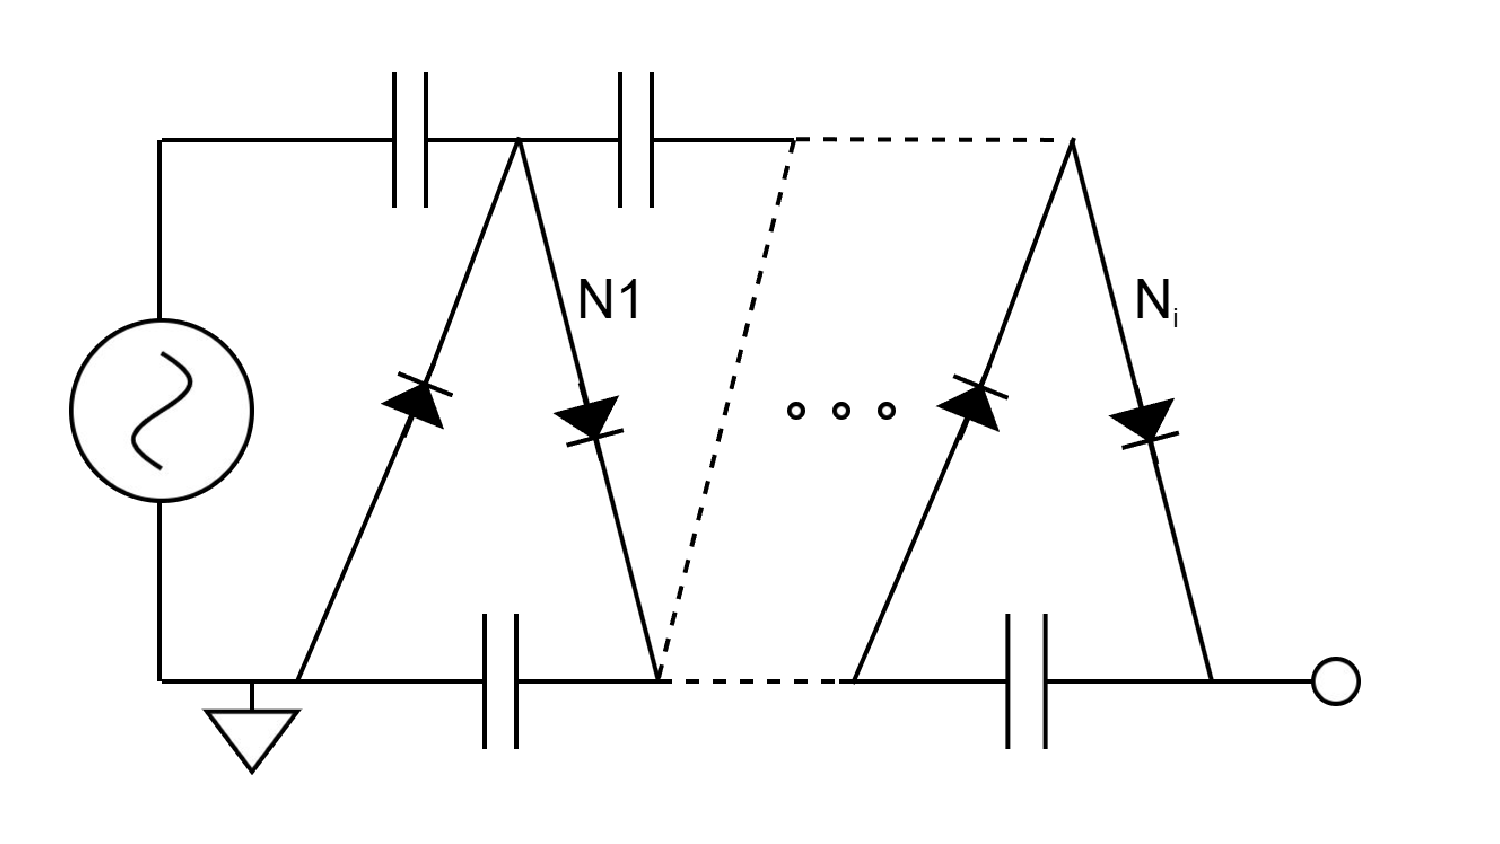
\includegraphics[width=\linewidth]{B/cockcroftwaltercircut.pdf} \caption{Circuit diagram of an N-stage Cockcroft-Walton multiplier, inspired by Refs. \cite{cockcroftwalton} and \cite{grdjournal}.} \label{fig
} \end{figure}

The CW multiplier converts a low AC input to a high DC output by employing a sequence of diodes and capacitors, which sequentially step up the voltage. This design ensures a stable and high terminal voltage for ion acceleration.
In the CW multiplier, each of the N stages consists of two capacitors and two diodes. The capacitors are charged in parallel, with every second capacitor in each stage connected in series between the ground and the output. This configuration results in an output voltage proportional to the number of stages, effectively multiplying the input voltage by an even factor.

The output voltage, $V_{out}$, is therefore given by:
\begin{equation} V_{out} = 2 N_{i} V_{in} \end{equation}
where $N_{i}$ is the number of stages and $V_{in}$ is the input voltage.

This terminal voltage creates the electric field that drives ion acceleration throughout the system, with field strength gradually decreasing at the extremities of the accelerator.

\subsection{Charge-exchange gas cell}
At AARAMS, the gas used in the stripper is typically argon, with the option to switch to helium via the dual gas stripper setup \cite{Klein2014}. Gas is preferred in the stripper to ensure stable beam transmission, especially when lower charge states are desired. In the stripping process, the negative ion beam is directed through a gas layer with a thickness of approximately \(1-2 \, \mu \text{g/cm}^{2}\), while minimizing gas diffusion into the low- and high-energy accelerator tubes. Excessive gas in these tubes can scatter the ion beam, potentially producing neutral particles, positive ions, and electrons that disrupt transmission efficiency, particularly if the vacuum is suboptimal. The low-energy tube is more susceptible to such interference, as the slower ions here are more prone to charge exchanges outside the stripper. To mitigate these issues, turbopumps maintain a high vacuum in the tubes, recirculating gas back to the stripping chamber.

If electrons produced through scattering are not directed to a tube electrode, they may gain enough energy to cause further collisions, leading to additional electron or ion production. The resulting X-rays can ionize the insulating gas, drawing charge from the multiplier and terminal rings to the tank wall, leading to voltage drops, known as electron loading. To control radiation levels, a bias ring set to \ce{-4$\kV$} is placed at the accelerator entrance to block incoming electrons.

In the LE section of the accelerator tube, ions reach a total energy at the stripper defined by
\begin{equation}
    E_{\text{strip}} = E_{i} + eV_{\text{TV}}
\end{equation}
where \(E_{i}\) is the initial ion energy, and \(V_{\text{TV}}\) is the accelerator's terminal voltage.

Upon entering the stripper, ions undergo two main processes: electron capture, which decreases the ion’s charge state \(\ce{q}\) by one as an electron is gained, and electron loss, where the ion loses an electron, increasing its charge state. These processes are represented by the reactions:
\begin{equation}
    Z^{q} + e^{-} \rightarrow Z^{q-1}
\end{equation}
and
\begin{equation}
    Z^{q} \rightarrow Z^{q+1} + e^{-}
\end{equation}
Each process has a specific probability based on cross-section, ion charge, excitation state, and kinetic energy. As ions move through the gas, they alternate between capture and loss, stabilizing into a quasi-pseudo-equilibrium charge state. This process allows various charge states for \ce{^{10}Be}, such as \ce{^{10}Be^{q+1}} and \ce{^{10}Be^{q+2}}. Diagram illustrating the charge-exchange process for a negative ion (q = -1) as it passes through a stripping gas or foil. A schematic of this is shown in \cref{fig:hargestateequlibrium}, the vertical axis represents the charge state, the left horizontal axis shows the thickness of the stripping medium in arbitrary units, and the right horizontal axis indicates the fraction of ions in each charge state that has passed through the stripper.

\begin{figure}[ht]
    \centering
    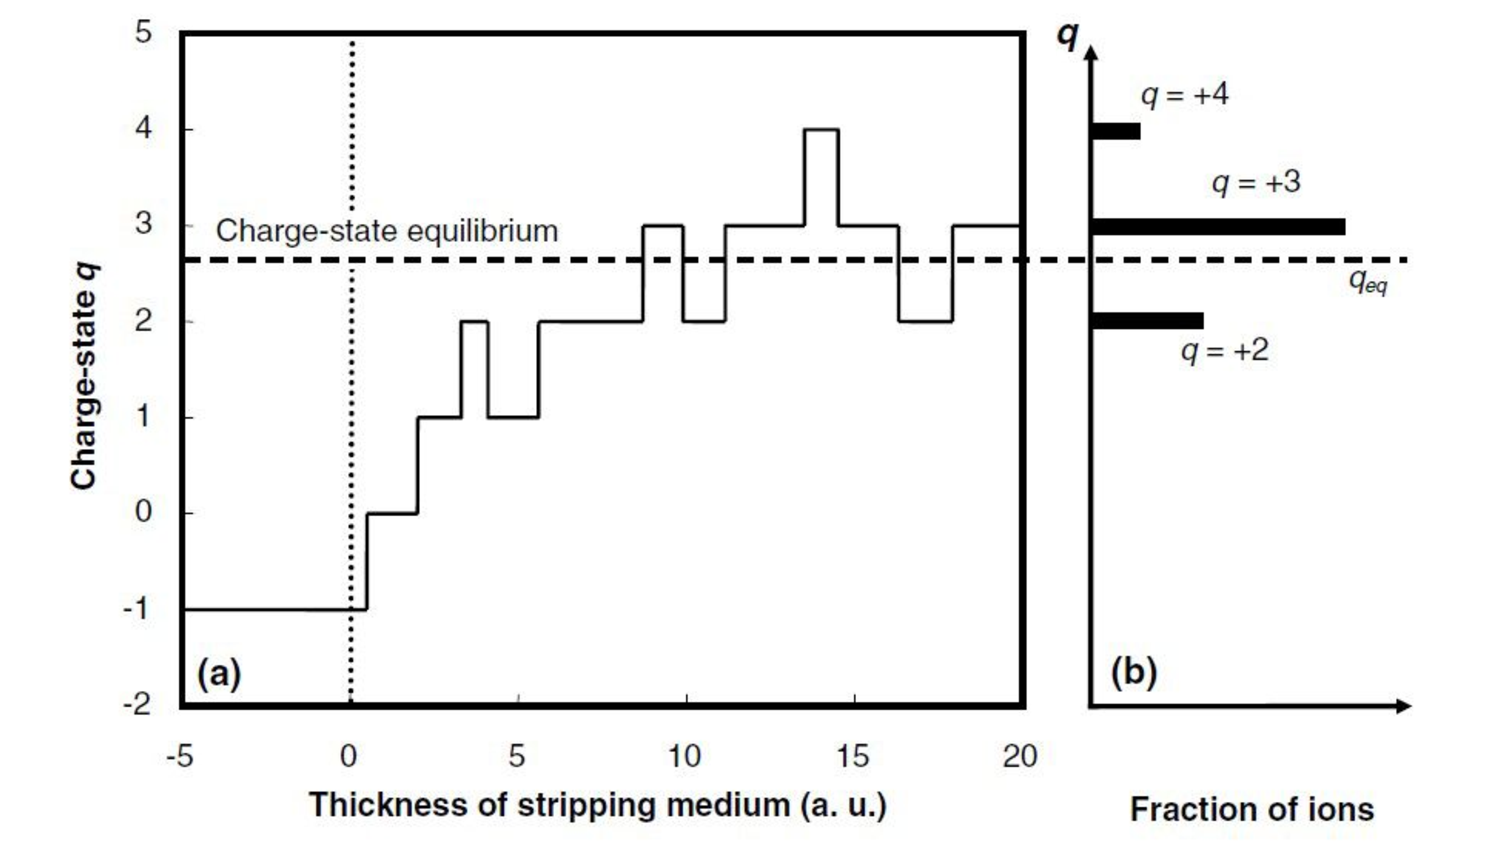
\includegraphics[width=1\linewidth]{B/chargestateequlibrium.pdf}
    \caption{Stepwise exchange is shown schematically for an ion of charge $q=1$ Ref. \cite{Whitlow2005}.}
    \label{fig:hargestateequlibrium}
\end{figure}



Although the stripper is a minor component of the AARASM, it plays a crucial role and requires precise handling. Stripper gas pressure is pivotal: it influences the efficiency of molecule ion dissociation but, if too high, may cause beam divergence due to angular scattering \cite{HVEE2013}. This effect can be mitigated to an extent by the Q-pole lens at the exit.

Optimizing the stripper gas cell pressure is essential to suppress unwanted background while maximizing the desired charge states of \ce{^{10}Be^{q}}. However, specifying the exit charge state with complete certainty is challenging due to the energy-dependent charge state distribution and the quasi-pseudo-equilibrium state, along with unavoidable scattering events.

Because of the low nuclear physics energy regime, high charge states \(q>5\) are not abundant and thus not a primary concern.

Neglecting potential energy loss, the energy of positive ions leaving the accelerator remains as given in \cref{ionenergyafteracc}.

Despite its critical function, the stripper poses challenges. Transmission measurements through the stripper are given as a function of thickness, \(\mu \text{g/cm}^{2}\), rather than pressure, and the stripper tube’s volume at AARAMS is unknown. To approximate thickness, we use the pressure gauges near the stripper to obtain terminal readings.

The stripper thickness can be calculated by integrating the local number density along the beam path:
\begin{equation}
    d = \int^{\infty}_{-\infty} \mu(x) \, dx
\end{equation}
Assuming constant pressure throughout the gas cell, we can simplify the thickness calculation using the ideal gas law. However, this approach overlooks potential leakage at the ends. To account for this, we approximate the local number density by assuming a constant pressure inside the cell and a gradual pressure decay outside, proportional to the cell radius and inversely proportional to the square of the distance. Thus, the effective thickness is estimated as
\begin{equation}
    d = A \frac{273.15}{273.15 \, T(\,^{\circ}\text{C})} \frac{P_{G}(\text{torr})}{760} \left( \ell + 2(r_{1}+r_{2})+(\ell_{1}-\ell)\frac{P_{1}}{P_{G}} \right)\label{stripperthicknes}
\end{equation}
where \(\ell, P_{G}, \ell_{1}, P_{1}\) denote the gas cell's length and pressure, and the first differentially pumped cylinder’s length and pressure. The pressure \(P_{1}\) is unknown due to the absence of a gauge at this location \cite{peterrømermøller}.

To use \cref{stripperthicknes}, we make an educated estimate between the terminal pressure and the LE tube's endpoint pressure reading. Dimensions are available from diagrams, but the temperature inside the cell remains unknown, as AARAMS lacks an internal sensor.

During the accelerator's startup, the pressure in the \(\text{SF}_{6}\)-filled tank increases to steady-state due to heating from the Cockcroft-Walton multiplier. Assuming ideal gas behavior, the temperature increase can be calculated as follows:
\begin{equation}
    \frac{P_i}{P_f} = \frac{T_i}{T_f}
\end{equation}
where \((P_i, T_i)\) and \((P_f, T_f)\) represent initial and final pressures and temperatures. The initial tank temperature, assumed to match room temperature, is reasonable if the AMS system hasn’t been active for an extended time.



\subsection{HE Section}
The high-energy ion beam with energy given by \cref{higenergysection} leaves the accelerator. It now enters the $\ce{90^{\circ}}$ analyzing magnet, with a radius of \ce{850mm}, a gap of \ce{50mm}, and a mass-energy product of \ce{63-73 AMU-$\MeV$} in the HE section. 
The $\ce{90^{\circ}}$ HE magnet is shown on \cref{fig:HEAARASM.pdf}.
The increased energy of the ion beam will now require the magnetic-, and electric fields in filtering components, e.g. ESA, to be stronger compared to the latter sections

\begin{figure}
    \centering
    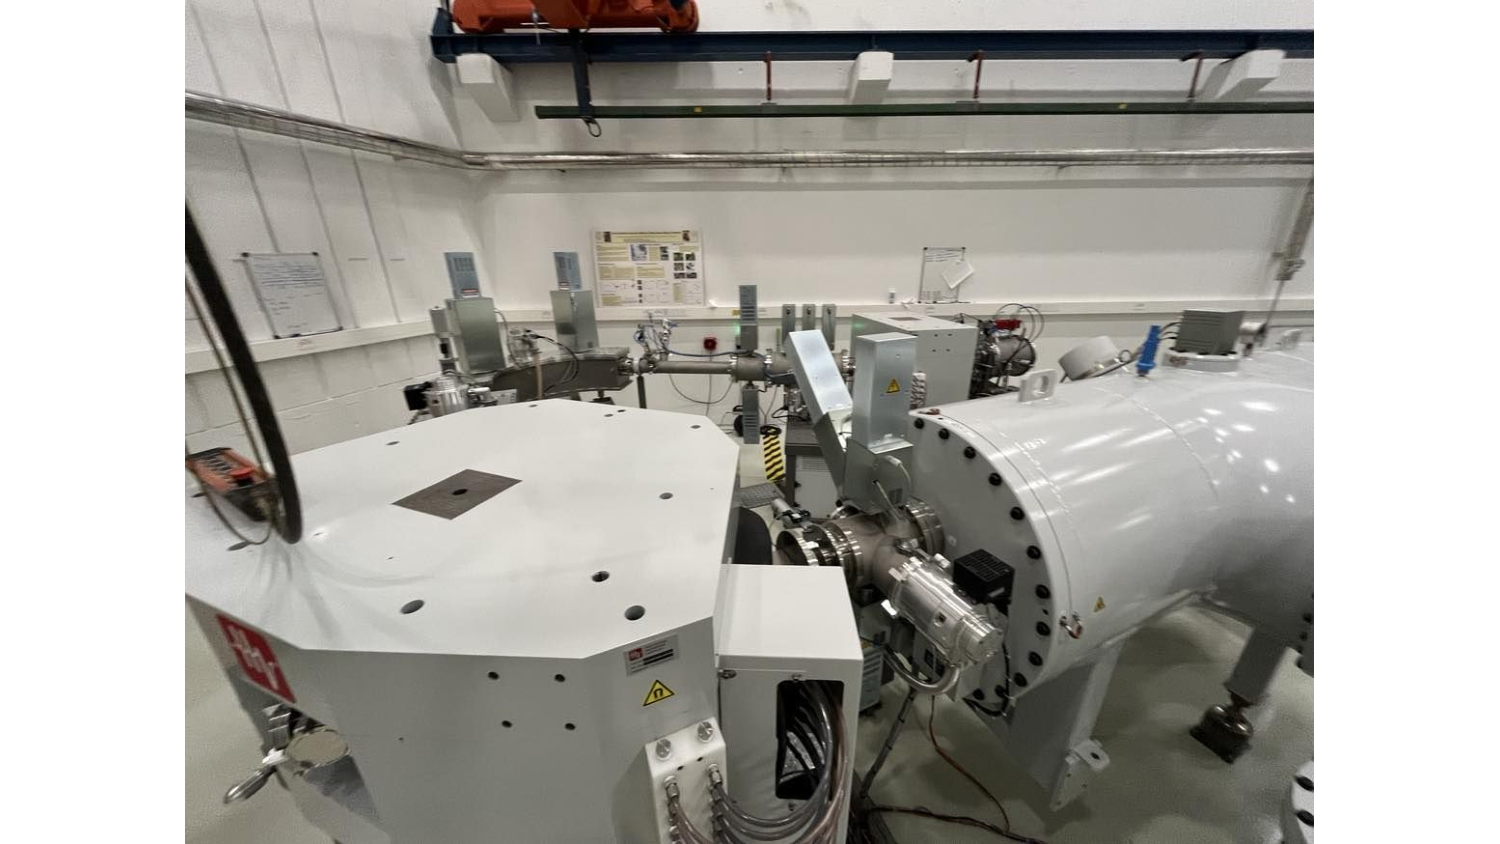
\includegraphics[width=1\linewidth]{B/HEAARASM.pdf}
    \caption{HE section at AARAMS from High Voltage Engineering Europa B.V.}
    \label{fig:HEAARASM.pdf}
\end{figure}

The HE magnet analyzes the ion beam according to a radius that can be isolated from \cref{magnetrigitidy}.

Molecules such as \ce{^{10}Be^{16}O} will be dissociated in the stripper, and therefore the mass of some ions will have changed. The function of the magnet is to guide the trajectory of \ce{^{10}Be}, as well as \ce{^{10}B}, the \ce{^{9}Be} will be separated and measured in offset Faraday cups after the magnet. 
The ion beam will continue toward the RI section. Additionally, the Faraday cup used to measure the \ce{^{9}Be^{+}}-ion beam is equipped with two vertical slits (electrodes) that provide information about the beam's position within the cup. The signal generated by these slits can be utilized in a feedback loop to stabilize the terminal voltage of the accelerator, ensuring that the rare isotope beam enters the ESA in the RI section at a precisely defined and reproducible location Ref.\cite{HVEE2013}. This is illustrated in \cref{faradaycupslits} which is from Ref.\cite{Kovalchuk2015}.

\begin{figure}[ht]
    \centering
    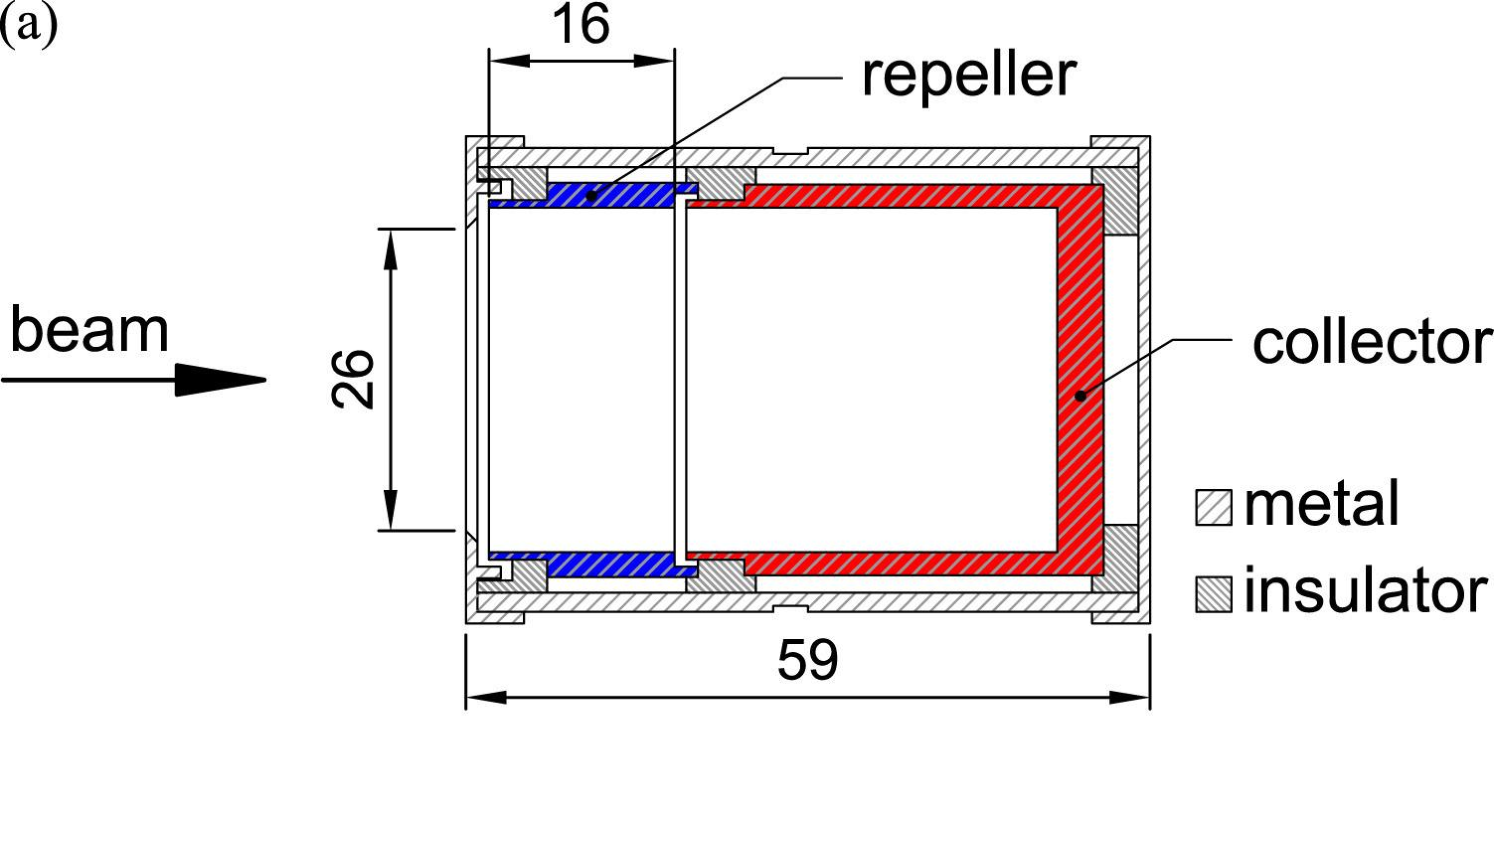
\includegraphics[width=\linewidth]{B/FCCERN.pdf}
    \caption{Standard Faraday cup utilized in REX-ISOLDE. Cross-sectional view of the standard REX-ISOLDE Faraday cup, with distances indicated in millimeters.}
    \label{faradaycupslits}
\end{figure}


\subsection{RI Section}
The last section before the detector is the rare-isotope section. The main components the ion beam will traverse are the $\ce{120^{\circ}}$ ESA and the $\ce{30^{\circ}}$  magnet before reaching the ionization chamber section (GIC).

We use an Electrostatic Analyzer (ESA) with a deflection angle of \(120^{\circ}\), a radius of 650 mm, a gap of 25 mm, and an energy-to-charge ratio of 1.5$\MV$. Although this ESA removes many unwanted particles, some isobars may still pass through due to their increased energies. To further refine the beam, it is directed through a second ESA before passing into a \(30^{\circ}\) magnet with a radius of 850 mm, a gap of 40 mm, and an energy-to-charge ratio of 63 AMU-MeV, with a maximum tolerance of 73 AMU-$\MeV$. This additional magnetic filtering step ensures even greater suppression of background particles and unwanted ions that might have scattered off the ESA electrodes, enhancing the purity of the final beam.


\subsection{Detector}

The detector is a gas ionization chamber filled with isobutane that operates as follows:

Upon entering the chamber through a thin foil-covered window, a beam of cations traverses the detector’s gas volume. As the ions pass through the gas, they collide with isobutane molecules, losing energy until they come to a complete stop. This energy loss, referred to as the stopping power, is the key measurement of the detector and is expressed as the energy loss per unit path length - \( \frac{dE}{dx} \).

Most of the ion energy is used to produce electron-ion pairs in the gas, a process called electronic energy loss, with a negligible fraction converted to thermal energy. This energy loss mechanism is described by the Bethe-Bloch equation \cite{sigmund2006}, which models the electric field generated by a moving particle as follows:

\begin{equation}
    E = \frac{Ze}{4 \pi \epsilon_0} \frac{1}{b^2}
\end{equation}

where \( Z \) is the atomic number of the ion, \( e \) is the elementary charge, and \( b \) is the impact parameter. By integrating over all relevant impact parameters, we can calculate the total energy loss per unit length, by summing the energy transferred to electrons at various distances. If \( n \) is the electron density in the isobutane, the number of electrons within a radius \( b \) and thickness \( db \) is \( 2\pi b \, db \, n \). Applying classical and quantum mechanical limits yields the following non-relativistic expression for the energy loss:

\begin{equation}
    \left( \frac{dE}{dx} \right)_e = \frac{4 \pi Z^2 e^4}{m_e v^2} n \ln{\left( \frac{2 m_e v^2}{I} \right)}
\end{equation}

where \( v \) is the particle velocity, $v=c\sqrt{1-\left(Ac^{2}/E+Ac^{2}\right)^{2}}$, \( m_e \) is the electron mass, \( c \) is the speed of light in vacuum, and \( I \) is the mean excitation energy. In high-energy regimes, energy loss scales as \( \frac{AZ^2}{E} \), while at low energies, incomplete stripping of the ion’s electrons results in a decreasing \( \frac{dE}{dx} \).

A schematic of the GIC is shown in \cref{fig:GICdrawing}. As the ion beam travels through the gas, it splits isobutane molecules into electron-ion pairs, which are separated by an electric field, electrons drift toward the anodes and ions toward the cathode. The number of electron-ion pairs produced is proportional to the ions' energy loss.

\begin{figure}[ht]
    \centering
    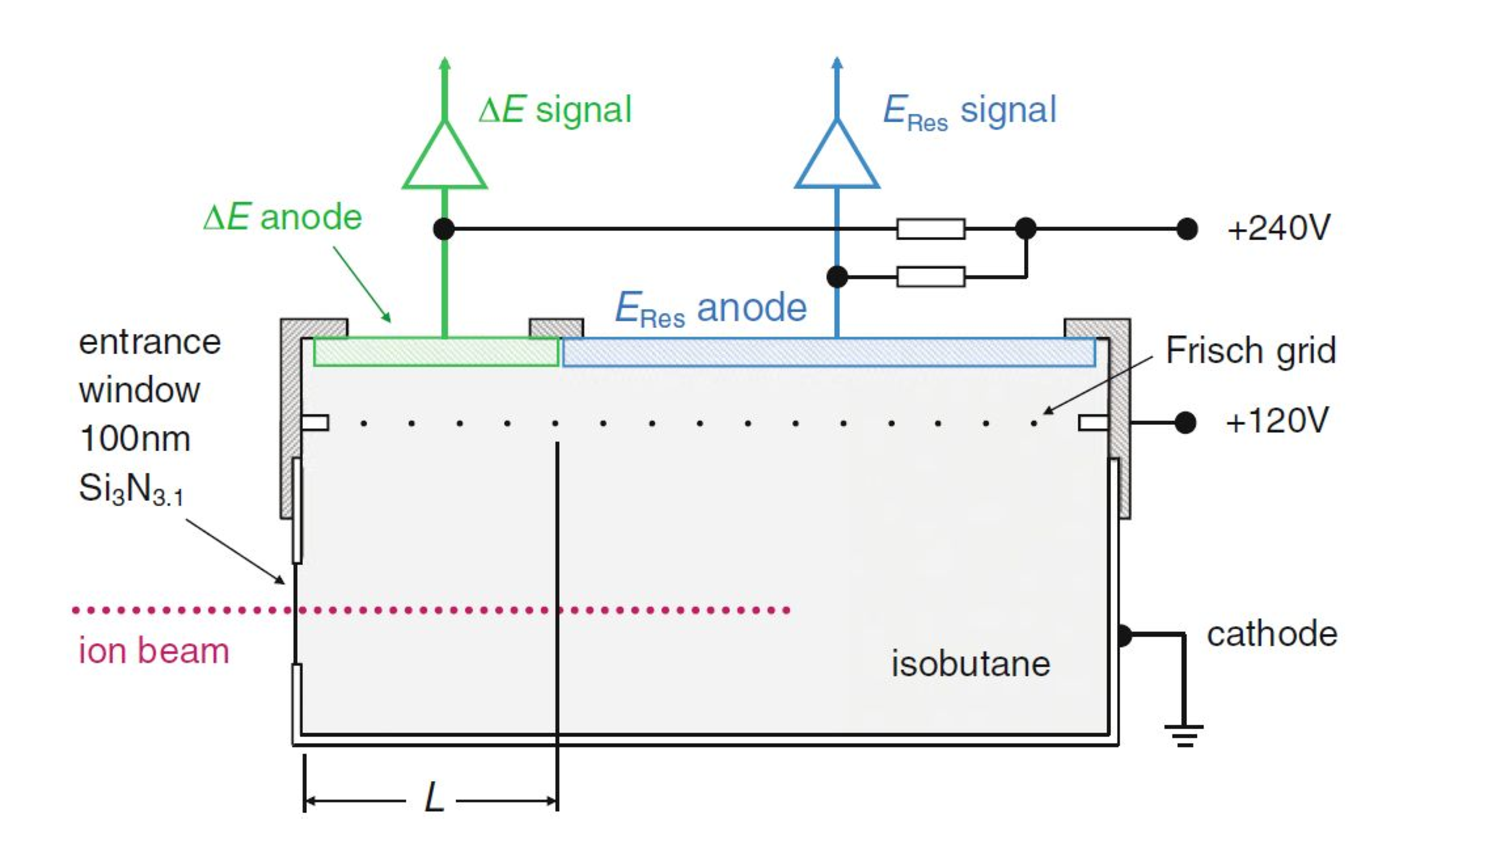
\includegraphics[width=1\linewidth]{B/GICdrawing.pdf}
    \caption{Schematic of an ionization chamber detector with a two-part anode, adapted from Ref \cite{steinhof2016}. Each section of the anode collects electrons from the sensitive volume beneath it. The $\Delta E$-anode's sensitive volume is defined by length \( L \). A Frisch Grid is positioned between the ionization region and the anodes.}
    \label{fig:GICdrawing}
\end{figure}

Due to their higher mobility, electrons reach the anodes faster than ions, which effectively makes ions appear stationary during electron collection. The Frisch Grid, located between the anodes and the cathode, minimizes positional and drift velocity effects by allowing only electrons that pass through it to generate a signal on the anode.

The data acquisition system collects signals from the two anodes, $\Delta E$ and $E_{res}$, in a two-dimensional manner, amplifying each signal independently.

The detector is designed with electric fields perpendicular to the anodes, ensuring each anode collects electrons only from the volume directly below it. The signal from the first anode is proportional to the integral of the electronic energy loss over the length \( L \):

\begin{equation}
    \Delta E \propto \int_0^L \left( \frac{dE}{dx} \right)_e \, dx
\end{equation}

where \( L \) is the length of the $\Delta E$ region along the beam direction. The second anode, long enough to capture all remaining ions, measures the residual energy:

\begin{equation}
    E_{res} \propto \int_L^\infty \left( \frac{dE}{dx} \right)_e \, dx
\end{equation}

Simultaneous measurements of energy loss and residual energy enable the determination of an ion’s nuclear charge \( Z \), which varies for isobars like \ce{^{10}Be} and \ce{^{10}B} due to their differing energy loss profiles in isobutane.

The ideal length of the $\Delta E$-anode is set by identifying the crossing point in energy loss curves as a function of penetration depth for different ions. From these measurements, $\Delta E$ and \( E_{res} \) can be obtained by analyzing intersections in energy loss curves.

Differences in signal help distinguish between ions, depending on the detector's resolution and the applied energy.

The signal, displayed as energy, is typically recorded as a channel number, which can be calibrated for a known isotope, such as \ce{^{10}Be}. To enhance the detection of \ce{^{10}Be}, blank-\ce{^{10}Be} samples can be measured as references.

A critical factor for detector performance is the isobutane gas pressure, as it affects both resolution and detection count. Pressure impacts the signals recorded on each anode and influences ion separation. High pressure stops ions sooner under the first anode, potentially complicating ion differentiation, while low pressure may prevent full ion stopping, lowering the count. Optimal pressure is achieved when energy distribution between the two anodes is balanced for the isotope of interest.


\section{Setups}
As shown in \cite{steier2019}, the overall ion detection efficiency for the degrader foil technique was 15$\%$, approximately one-third of the 45$\%$ achieved with the \ce{SiN} foil stack method. Building on this, we will determine the efficiencies of the degrader foil and \ce{SiN} stack methods using our setup and compare their performance. We are interested in reproducing similar findings for the 1MV tandem accelerator at AARAMS, see \cref{tab:comparison}.

\begin{table}[ht]
    \centering
    \caption{A comparison of the performance parameters for the three isobar suppression methods used at VERA in \ce{^{10}Be} detection. The overall ion detection efficiency refers to the detection efficiency from the anion beam in the ion source to the final \ce{^{10}Be} detection, excluding the ionization yields of the sputter source.}
    \label{tab:comparison}
    \resizebox{\linewidth}{!}{%
        \begin{tabular}{@{}lccc@{}}
            \toprule
            \textbf{Parameter} & \textbf{Degrader Foil} & \textbf{Gas Absorber} & \textbf{Foil Stack} \\ 
            \midrule
            Overall ion detection efficiency      & 15\%  & 5\%   & 5\%   \\
            Stripping yield \& acceler. transm.  & 55\%  & 5\%   & 55\%  \\
            HE-transm. \& detector efficiency    & 28\%  & >90\% & >80\% \\
            Reproducibility for identical sputter targets, $^{10}$Be/$^9$Be > $10^{-12}$ & 3\% & 1\% & 1\% \\
            Blank level $^{10}$Be/$^9$Be         & $(2+4/-2) \times 10^{-16}$ & $1 \times 10^{-14}$ & $<7 \times 10^{-16}$ \\
            \bottomrule
        \end{tabular}%
    }
\end{table}




\subsection{Degrader technique}


\subsection{Absorber technique}
beskrivelse af
***Beskrivelse af nye opstilling samt hvad vi forventer +  hvad har vi tænkt at gøre vis den nye tekiske tegning af dims + hvad var min geniiale ide***

***
Geniale ide - bruge slits før beam bliver afbøjet ind I RI
***

\section{SRIM Simulations}
\newpage